\documentclass[10 pt]{article}

\usepackage[a4paper, margin=1in]{geometry}


\usepackage{graphicx}
\usepackage[export]{adjustbox}
\graphicspath{
{./graphs/} }
\usepackage{subcaption}
\usepackage{mathtools}
\usepackage{hyperref}

\title{A study of different flowering strategies in response to vernalization}
\author{Gurpinder Singh}
\date{}
\begin{document}

\maketitle

This report presents the results from my implementation of a genetic-physiological model of flowering in \textit{Arabidopsis}, originally developed by Prof. Akiko Satake. In this project, I implemented the model equations in Python and obtained the solutions for a toy temperature dataset function. The results obtained in this implementation are similar to that obtained by the author in the original study. Parameters of the model were changed a bit to account for the change in the data between this implementation and the original study. The actual code and the parameters can be found in the Jupyter notebook.     

\section{Introduction}

Vernalization is the process by which plants transition from vegetative state to flowering state after exposure to prolonged period of cold temperature. Plants have the ability to filter out daily changes and variations in the temperature (noise) and obtain a stable long term estimate of the temperature trends. This allows the plants to adapt to different environments and seasons. Interestingly, this process results in various life cycles or flowering strategies depending upon the plant's response to the prolonged cold winters. \\

FLOWERING LOCUS C (FLC) is a transcription factor that acts as a flowering repressor and VERNALIZATION INSENSITIVE 3 (VIN3) is one of the initial repressors of FLC during winters. The repression of FLC activates FLOWERING LOCUS T (FT), which leads to production of FT protein. FT protein is then transported from leaves to the shoot apical meristem, where it initiates flowering. \\

The model takes into account the dynamic interactions between VIN3, FLC transripts and FT protein concentrations in response to the cold temperature. The model also assumes that the repression signal is digital in nature, i.e. the FLC activity in the cells is either repressed or activated. There are many known transcription factors in the actual gene regulatory network along with the photoperiod pathway, which are ignored in this particular model.  

\section{Temperature dataset}

The temperature dataset that was originally used in the study could not be located for this implementation. Thus, I developed a simple model to generate a random temperature dataset array for any number of days. This allows fine control over the temperature parameters that one wants to run the simulation for, such as the average temperature, temperature range and the amount of noise.  
\begin{equation}\label{temp_eqn}
\theta(i) = \theta_{av} + \theta_{r} \sin\bigg(\Big(M(i) + \frac{D(i)}{30} \Big)\frac{\pi}{12}\bigg) + \theta_{n}
\end{equation}

The equation \ref{temp_eqn} is the trignometric function used to generate temperature data in this study, where $\theta(i)$ is temperature for any $i^{th}$ day, $\theta_{av}$ is the average temperature, $\theta_{r}$ is the temperature range, $M \in [0,11]$ and $D \in [0,29]$ are the month and day number respectively. $\theta_{n} \sim \mathcal{N}(\mu, \sigma)$ is the gaussian noise, with mean $\mu$ and variance $\sigma$. 

For simplicity, every month is assumed to have 30 days.
\pagebreak

\section{Summary of the model}

As described by Prof. Akiko Satake, the model focuses on the vernalization pathway and showcases the repression of FLC due to prolonged cold temperatures (below the vernalization threshold in the model, $K_{T}$) and its subsequent maintenance. The principal FLC repressor (in the model), VIN3 expression, is induced by the cold temperature. 
\begin{equation} 
\label{eqn1a}
\frac{dX_{VIN3}}{dt} = \beta_{v}\theta(T(t) \ge K_{T}) - \alpha_{V} X_{VIN3}
\end{equation}

\begin{equation} 
\label{eqn1b}
	\theta(T(t) \ge K_{T}) = \begin{dcases}
								 1 & \rm{if} \: T(t) \ge K_{T}\\
								 0 & \rm{otherwise}		
								\end{dcases} 
\end{equation}

In equation \ref{eqn1a}, $\beta_{V}$ is the production rate of VIN3 transcripts and $\alpha_{V}$ is the degradation rate for the same. $X_{VIN3}$ is the number of the VIN3 transcripts. $\theta(T(t) \ge K_{T})$ is a step function as described by the equation \ref{eqn1b}.

VIN3 expression leads to increased repressive histone modifications at FLC locus and a decrease in modifications associated with active transcription. In the original study the cells were assumed to be either repressed or active i.e the repression signal is analogus to a digital signal. $R_{FLC}$ are the fraction of the cells that are in repressed state. 

\begin{equation} 
\label{eqn: eqn2}
	\frac{dR_{FLC}}{dt} = q \theta(X_{VIN3}(t) < K_{VIN3}) (1 - R_{FLC}) - p R_{FLC}
\end{equation} 

$R_{FLC}$ changes according to equation \ref{eqn: eqn2}, in which, the parameters p and q are the rates at which repressive cells change to active state and the rate at which active cells change to repressed cells respectively. Changing these two rates, while keeping all other parameters fixed produces different flowering strategies.

FLC transcript level per unit leaf biomass depends on the fraction of cells that are in repressed state. The maximum transcript level is denoted by $r$. 
\begin{equation} \label{eqn3}
FLC(t) = r(1-R_{FLC}(t))
\end{equation}

Based on the transcript levels of FLC, if they are below a threshold level, FT protein concentration per unit leaf biomass changes.
\begin{equation}\label{eqn4}
\frac{dFT}{dt} = \beta_{FT}\theta(FLC(t) < K_{FLC}) - \alpha_{FT}
\end{equation}
where, $\beta_{FT}$ is the production rate and $\alpha_{FT}$ is the degradation rate of FT protein and $K_{FLC}$ is the threshold for FT protein production. 

In the model, it is assumed that the plants start bolting when, 
$xFT > K_{FT}$,
where x is the size of the total biomass and it changes according to,
\begin{equation} 
%\label(eqn5)
\frac{dx}{dt} = h[1-\theta(xFT > K_{FT})] \frac{ax}{1+bx} - d_{x}x,
\end{equation}
where, $h$ represents the fraction of the carbon gain used for vegetative growth and $\frac{ax}{1+bx}$ represents carbohydrates gained after subtracting the maintenance costs of plants. $d_{x}$ is the natural loss of biomass due to disturbances. The amount of stored resources (S) changes as,
\begin{equation} 
%\label(eqn6)
\frac{dS}{dt} = (1-h[1-\theta(xFT > K_{FT})]) \frac{ax}{1+bx} - C_{f} \theta(xFT > K_{FT}) - C_{s}y - d_{s}S,
\end{equation} 
where, $C_{f}$ indicates the rates of resources investment to produce flowers, $C_{s}$ is the rate of resource investment to produce fruits and seeds while $d_{s}$ is the resource investment for respiration. These three terms are subtracted from the main term that represents the resource investment by photosynthesis. The number of fertilized flowes changes according to,
\begin{equation}
\frac{dy}{dt} = \frac{C_{f}\theta(xFT > K_{FT})}{u_{f}} - d_{y}y,
\end{equation}
where, $u_{f}$ is the unit cost to produce a single flower. \\
For more details on the model, refer to the original paper in the references. Another book chapter by Prof. Akiko Satake (in references) is also an equally good read.

\section{Results}

The equation \ref{temp_eqn} was used to generate the temperature dataset array to obtain solutions to the differentail equations of the model. 

\begin{figure}[h]
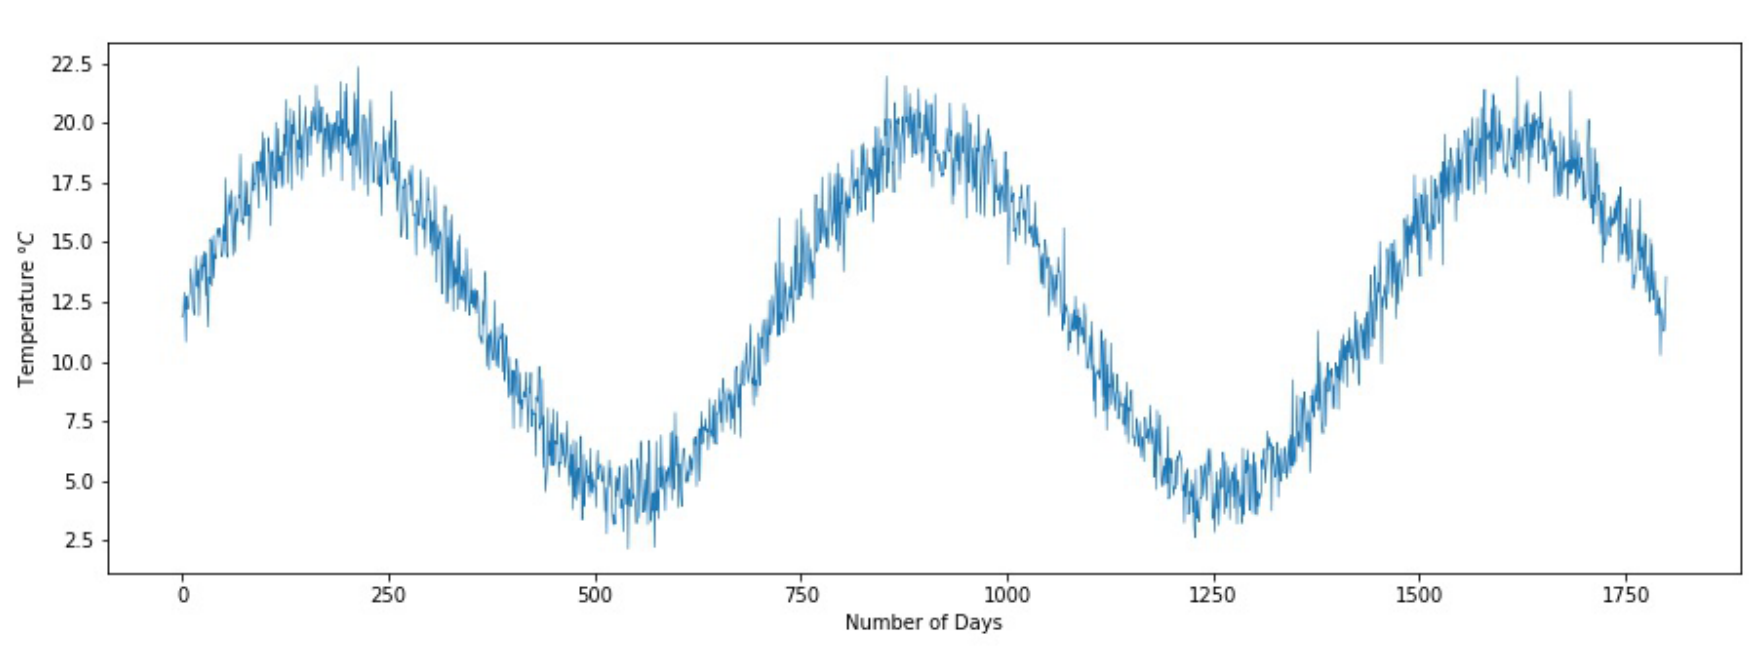
\includegraphics[width=0.9\textwidth]{Temp_1.png}
\caption{The data genrated by implementing equation \ref{temp_eqn}, for $\theta_{av}$ = 12, $\theta_{r}$ = 7.5, $\mu$ = 0, $\sigma$ = 2 for 60 months.}
\end{figure}

My implementation of the model yielded similar results to that of the original study. Here, I present 4 different flowering strategies produced by changing the values of parameters $p$ (rate at which repressed cells change back to active state) and $q$ (rate at which active cells are repressed).

For $p$ = 0.0 and $q$ = 0.2, i.e. when cells once repressed, stay repressed; \textbf{Monocarpic} flowering strategy was observed. Here, plants retain the ``winter memory'', i.e. even after the temperature rises above the vernalization threshold, (here, $K_{T}$ = 10$^{\circ}$C) and VIN3 transcript level drops to zero, FLC stays repressed. These monocarpic plants require only one winter to flower and thus can be classified as \textbf{Monocarpic annuals}, however, here the temperature dataset is from a plant where one year spans about 600 days. 
\begin{figure}[h]
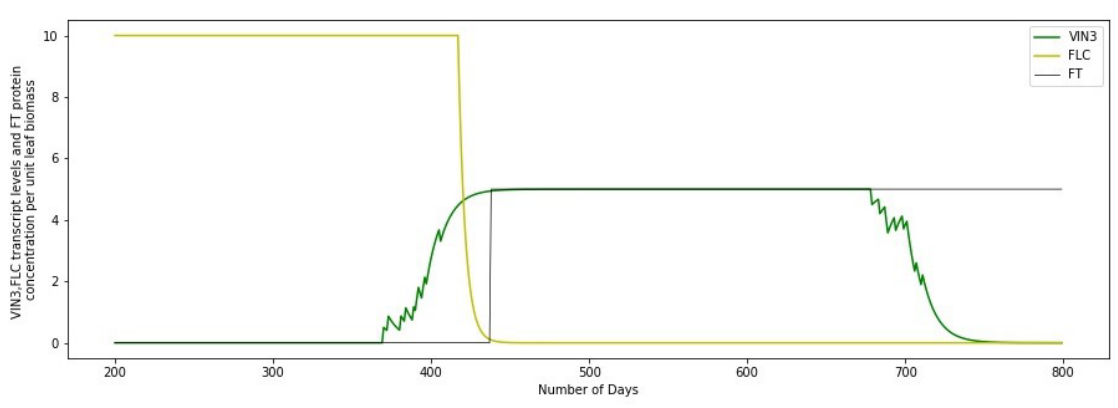
\includegraphics[width=0.9\textwidth, left]{annual_vin-flc.png}
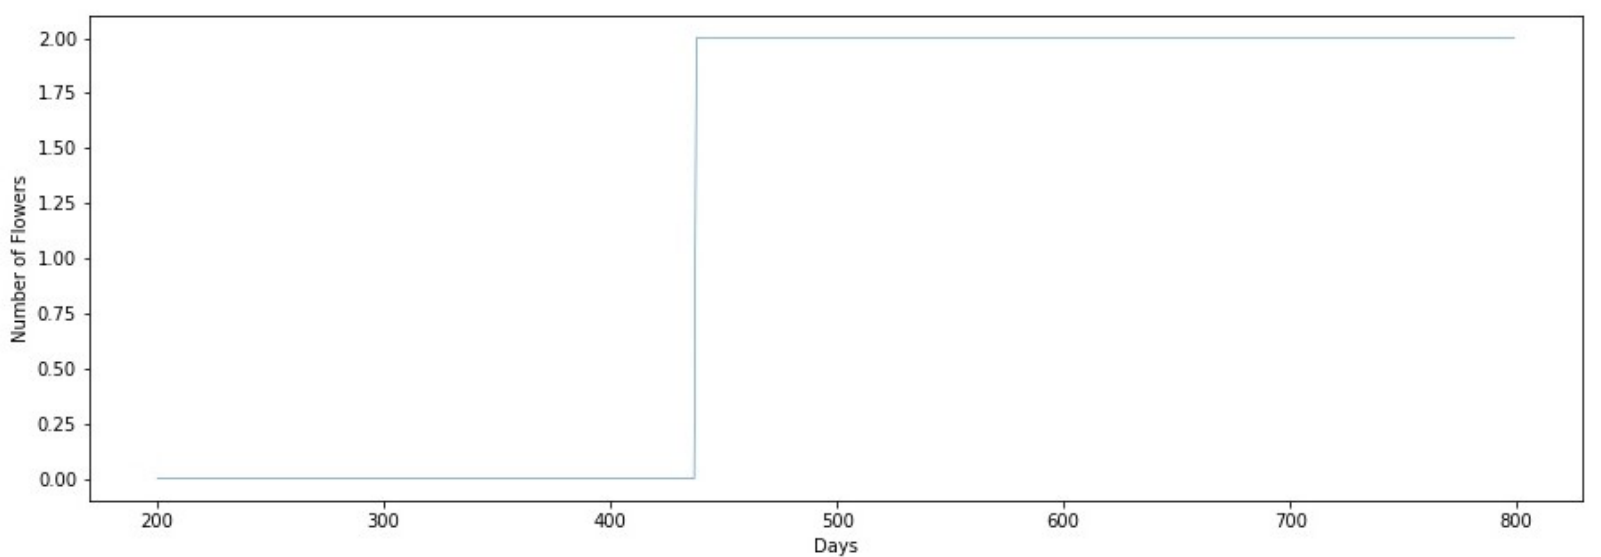
\includegraphics[width=0.9\textwidth]{annual_flowering.png}
\end{figure}
\pagebreak

For $p$ = 0.0 and $q$ = 0.01, i.e. when rate of repression is very low, plants require more than one winter season to accumulate the reduction in FLC expression. This results in \textbf{Monocarpic perennial} flowering pattern.
\begin{figure}[h]
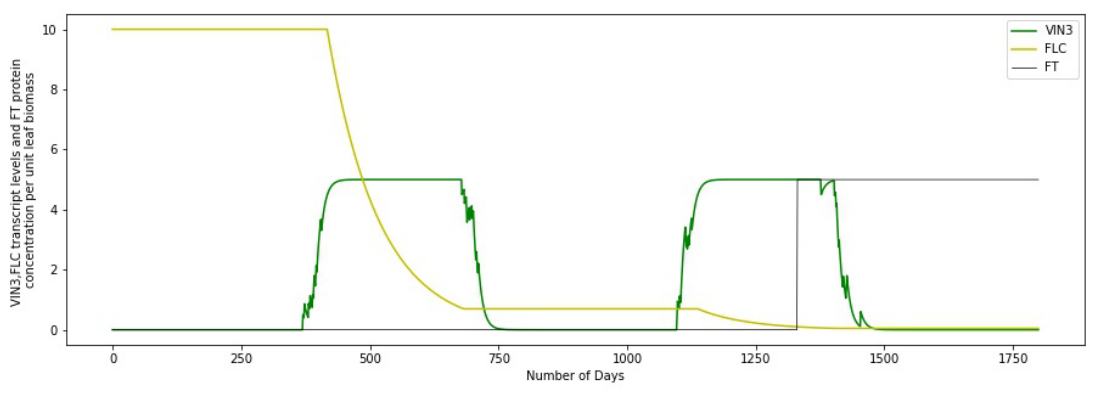
\includegraphics[width=0.9\textwidth]{perennial_vin-flc.png}
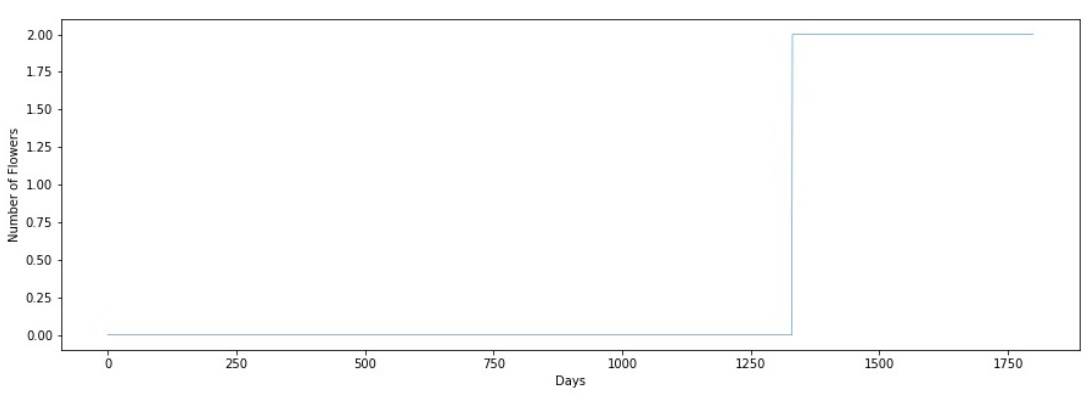
\includegraphics[width=0.9\textwidth]{perennial_flowering.png}
\end{figure}

For $p$ = 0.0072 and $q$ = 0.98, that is the cells once repressed for FLC, can become active after the winter, thus here, the winter memory is not stable. This results in \textbf{Polycarpic yearly} flowering. Here, the activation rate of FLC is not negligibly small. 

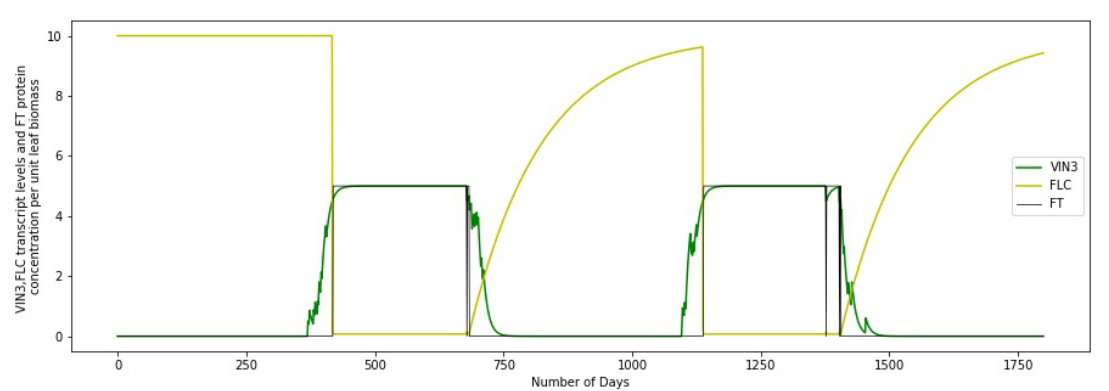
\includegraphics[width=0.9\textwidth]{perennial_poly_vin-flc.png}

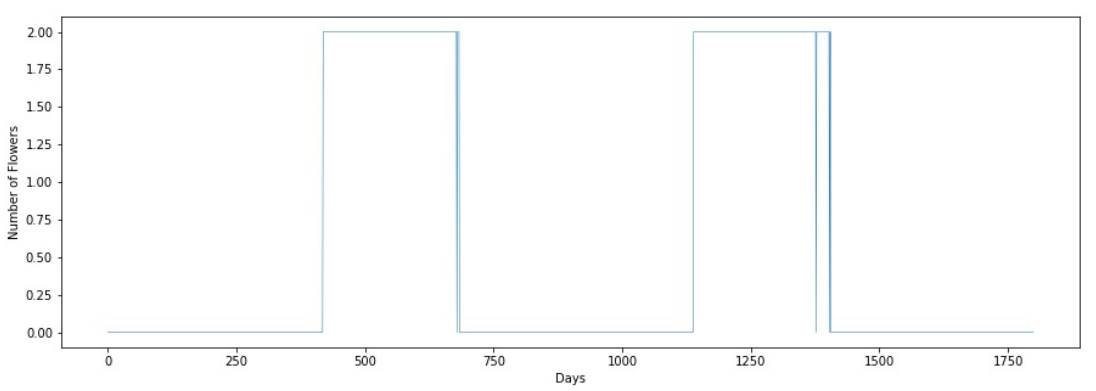
\includegraphics[width=0.9\textwidth]{perennial_poly_flowering.png}

Finally, for $p$ = 0.00089 and $q$ = 0.11, i.e. when rate of repression of FLC activity is not high enough. In such a scenario, whenever a warm winter occurs, as shown in this toy temperature signal, FLC expression is not repressed enough for flowering. This type of flowering behaviour can be classified as \textbf{Polycarpic intermittent}

\begin{figure}[h]
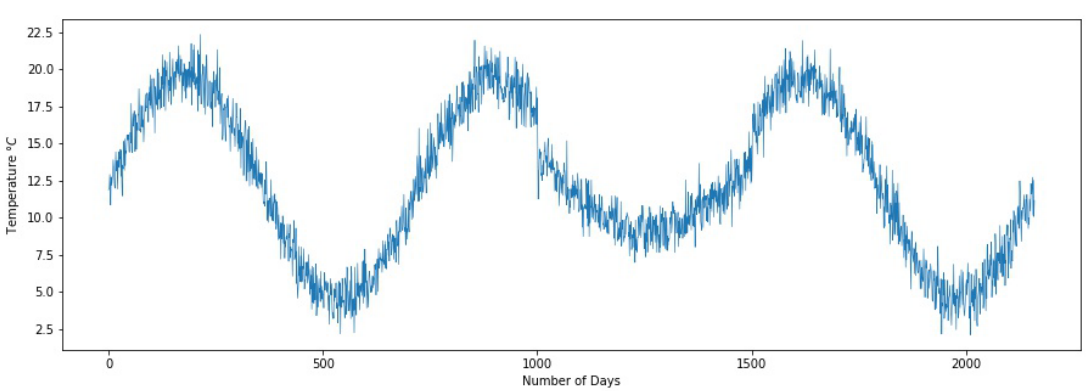
\includegraphics[width=0.9\textwidth]{polycarpic-intermittent-Temp.png}
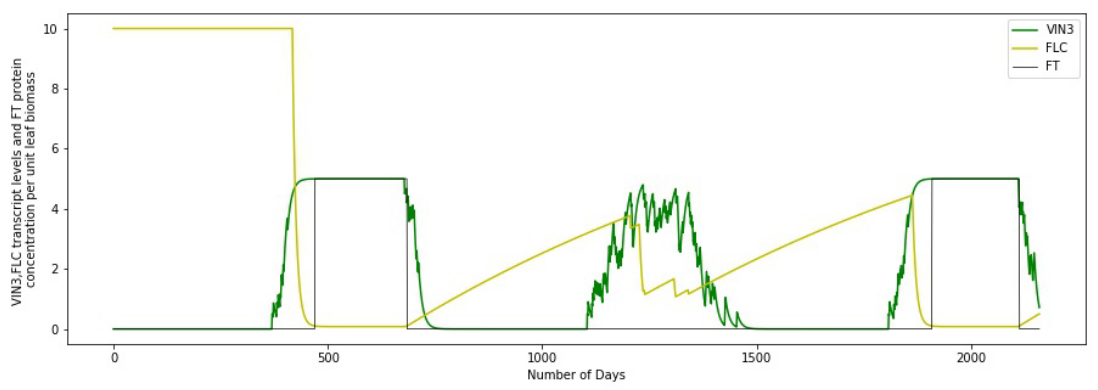
\includegraphics[width=0.9\textwidth]{polycarpic-intermittent-vin-flc.png}
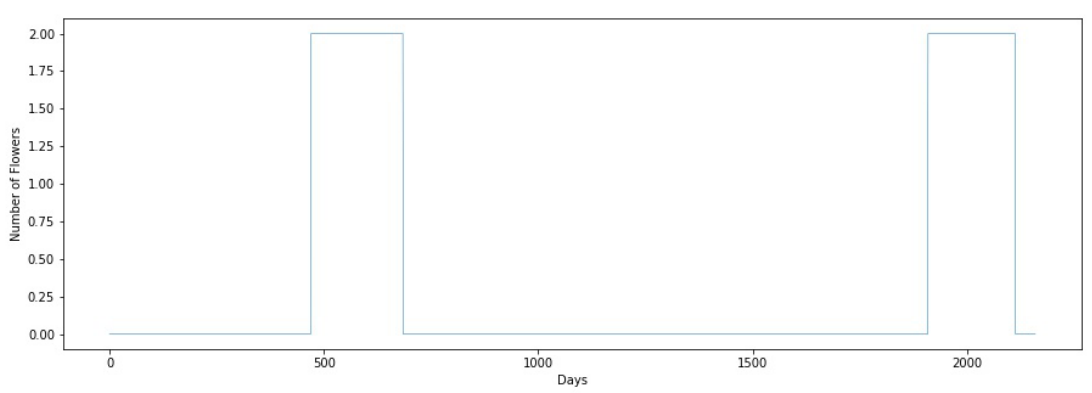
\includegraphics[width=0.9\textwidth]{polycarpic-intermittent-flowering.png}
\end{figure}


\section{Conclusion}

Flowering time is an interesting trait to study from both pure basic scientific point of view as well as from applied agricultural aspects such as crop varietal development. Insights from model plants such as \textit{Arabidopsis} serve as a starting point for subsequent studies in more complex crop species.

The model implementation clearly shows that different flowering strategies arise by changing the rate at which FLC expression in cells is repressed or reactivated once the temperature rises above the vernalization threshold again. This also shows evolution of plant life cycles depends upon the temperature. 

One interesting fact to note is that the repression signal is digital in nature, i.e. cells are either repressed or activated. If the repression rate ($p$) is very small, as in \textbf{Monocarpic perennial} flowering, the plants remember the fraction of reduction in FLC througout the summer. Such reduction is passed on in a digital manner, for the fraction of cells which are repressed, all the cells that are subsequently originate from them retain the FLC repression with a rate $q$ in the model.

The differential equations were implemented in python inside of a Jupyter Notebook.

\section{References}

Satake A., Diversity of plant life cycles is generated by dynamic epigenetic regulation in response to vernalization, Journal of Theoretical Biology, 266 (2010) 595 - 605\\% \href{https://doi.org/10.1016/j.jtbi.2010.07.019}{doi.org/10.1016/j.jtbi.2010.07.019}
Satake A. (2018) Flowering Time as a Model Trait to Bridge Proximate and Evolutionary Questions. In: Morris R.(eds) Mathematical Modelling in Plant Biology. Springer, Cham%\href{https://doi.org/10.1007/978-3-319-99070-5_9}{doi.org/10.1007/978-3-319-99070-5_9}
\end{document}
